\chapter{Team's Coordination}
\label{Coordination}

In this chapter, we are going to present the most important, exciting and time consuming part of this thesis. Until now, we have discussed all parts that agent is going to need in order to be functional into the soccer field.
With all these functionalities agents are able to locate themselves in the field, communicate with each other and execute actions combining movements through motion controller. However, agents miss a thinking process with which they will be able to decide about what action they should do for their team's benefit. For example, imagine a human soccer player who is able to do all the things needed in a football match but he has not the ability to choose what to do. Therefore, there must be presented a high-level process which will combine all these skills, motions,communication ability and actions having as a result a complete agent's behavior. As a behavior, we could define the process in which each agent takes as arguments his beliefs and decides what he will do as an output. In our approach, instead of each agent having his own behavior, players are depend on a centralized process which is called coordination.  Coordination's algorithm is responsible to gather messages from all agents and as an output it produces actions which are costless for all players who are included into this process. We chose goalkeeper as the coordination's administrator to be the one who is going to execute this procedure. This means that goalkeeper will only be ``running'' his own behavior and other field players will not. Field players are just sending their beliefs to the goalkeeper and he is sending back the actions which are calculated by the coordination's algorithm execution.
\begin{figure}[htb!]
\centering
  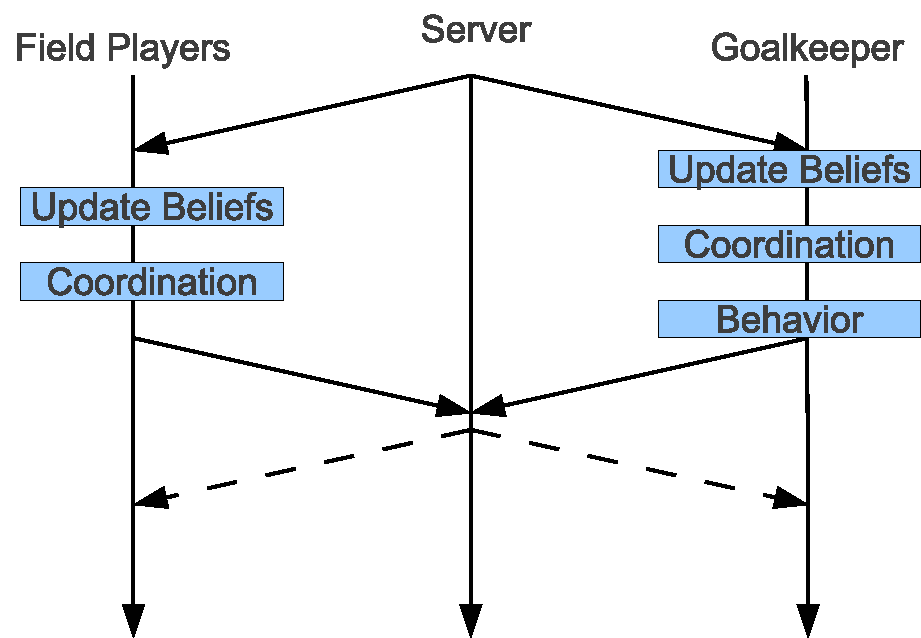
\includegraphics[width=0.6\textwidth]{Chapter4/figures/CoordinationCycle.pdf}
  \caption{Coordination cycle.} 
  \label{fig:CoordinationCycle}
\end{figure}


Figure \ref{fig:CoordinationCycle} shows the difference between a field player and the goalkeeper. Goalkeeper has to calculate actions for all field players as well as execute his own behavior. In contrast, field players do not execute any behavior but only send messages to goalkeeper and receive the calculated actions from him. We selected the goalkeeper to take the responsibility for this task due to the fact that he has the less significant role in the simulation soccer. Coordination's procedure is executed in several phases and not at once. These phases are:
\begin{description}
\item[Update coordination beliefs] Multiple world state beliefs from field players have to be combined in order to update our belief for the world state.
\item[Split field player into groups] Field players are split into groups according to their significance to the game state. The groups are:
\begin{description}
\item[Active] This group consists of three players and their responsibility is to support and protect the on ball player who is chosen by coordination to be the one who will be given an action which is related to the ball.
\item[Inactive] This group consists of players which are not able to know their positions in the field or they have been fallen on the ground.
\item[Support] This group consists of the team's rest players and their responsibility is to fill team's formation positions with the best way possible.
\end{description}
\item[Compute positions for active players] All possible positions which are best candidates for assigning active players there.
\item[Assign actions for active players] Computation of the best two positions according to their cost.
\item[Generate team's formation] Formation is generated according to ball's position.
\item[Assign roles for all players] Team players are assigned roles in relation to the team's formation and their current position.
\item[Find positions for support players] All possible positions which are best candidates for assigning support players there.
\item[Assign actions for support players] Computation of the best mapping  according its cost.
\end{description}


Algorithm \ref{CoordinationAlgorithm} describes the coordination procedure. In every cycle-step, only few of the above phases are executed. We chose doing that because of the time limitation of the think's cycle. So, in order to have a smooth algorithm's execution we decided to separate functions in a number of server cycles.

\begin{algorithm}[htb!]
\caption{Coordination Algorithm }
\label{CoordinationAlgorithm}
\begin{algorithmic}[1]
\STATE {\bf Input: }$Coordination Messages = \lbrace M_{1},M_{2},...,M_{N-1} \rbrace, N = number of players $
\STATE {\bf Output: }$Actions = \lbrace A_{1},A_{2},...,A_{N-1} \rbrace$
\IF {$ Step = 1$ }
\STATE $B \leftarrow Update Beliefs() $
\ELSIF {$ Step = 2$ }
\STATE $S \leftarrow Coordination Splitter(B) $
\ELSIF {$ Step = 3$ } 
\STATE $A_{p} \leftarrow Active Positions(B,S) $
\ELSIF {$ Step = 4$ }
\STATE $A_{c} \leftarrow Active Coordination(A_{p},S) $
\ELSIF {$ Step = 5$ }
\STATE $ F \leftarrow TeamFormation(B) $
\STATE $ R \leftarrow Role Assignment(A_{c},B,F) $
\STATE $ S_{p} \leftarrow Support Positions(R,F,S) $
\ELSIF {$ Step = 6$ }
\STATE $ Support Coordination(R,F,S,B,A_{c},S) $
\ENDIF
\end{algorithmic}
\end{algorithm}


\section{Messages and Communication}
Coordination could only be accomplished through communication. We use the common communication channel through simulation server in order to provide the messaging between players involved in coordination process. For this reason, communication plays a major role in our approach. 

\subsection{Message Types and Formats}
There are multiple types of messages, each one of them has a different functionality and serves an exact purpose. These message types are:
\begin{description}
\item[Init Message] This type of message declares the start of the coordination procedure for each agent into the field. All field players should sent this message to the coordination's administrator in order coordination procedure to begin.

\begin{description}
  \item[{\bf Message format:}]
  \begin{verbatim} 
  
  i,<Uniform number>
  \end{verbatim}
\end{description}

\item[Start Message] This type of message is only sent by the administrator, it declares that all agents are now initialized in the process. Each receiver of this message should immediately start sending coordination messages.

\begin{description}
  \item[{\bf Message format:}]
  \begin{verbatim} 
  
  s,<Uniform number>
  \end{verbatim}
\end{description}

\item[Coordination Message] This is the most important type message. It has information about each agent's beliefs. There are four types of these messages in respect to the agent's situation. these types are:
\begin{description}

\item[Type C] Agent has complete awareness of the world state. He sends his uniform number, his position and the ball's position accurately..

\begin{description}
  \item[{\bf Message format:}]
  \begin{verbatim}
  
  c,<Uniform number>,<Agent X>,<Agent Y>,
  <Ball X>,<Ball Y>
  \end{verbatim}
\end{description}

\item[Type L] Agent has complete awareness only for his position in the field, ball is not in his field of view and it could be best not to send us faulty observations about ball's position. He sends his uniform number and his position.

\begin{description}
  \item[{\bf Message format:}]
  \begin{verbatim}
  
  l,<Uniform number>,<Agent X>,<Agent Y>
  \end{verbatim}
\end{description}

\item[Type B] Agent has complete awareness only about the ball's distance from his body. its horizontal and its latitudal angle. He sends his uniform number,  and the ball's distance and angle in relation to his body angle.

\begin{description}
  \item[{\bf Message format:}]
  \begin{verbatim}
  
  b,<Uniform number>,<Ball Distance>,
  <Ball Horizontal-Angle>
  \end{verbatim}
\end{description}

\item[Type X] Agent has complete unawareness of the world state. He is sending only his uniform number.

\begin{description}
  \item[{\bf Message format:}]
  \begin{verbatim}
 
  x,<Uniform number>
  \end{verbatim}
\end{description}

\end{description}
\item[End Message]
This type of message serves to stop field players from sending coordination messages. In this step administrator of the coordination is ready to execute the procedure and calculate the actions for all field players.
\begin{description}
  \item[{\bf Message format:}]
  \begin{verbatim}
  
  e,<Uniform number>
  \end{verbatim}
\end{description}
\item[Action Message]
This type of message is only sent by the administrator, it declares which action an agent has been assigned by the coordination process. These messages are sent in the end of the coordination procedure when actions for all field players have been computed.
\begin{description}
  \item[{\bf Message format:}]
  \begin{verbatim}
  
  a,<Uniform number>,<Action ID>,<Action parameter1>,
  <Action parameter2>,<Action parameter3>
  \end{verbatim}
\end{description}

\end{description}

\begin{figure}[htb!]
\centering
  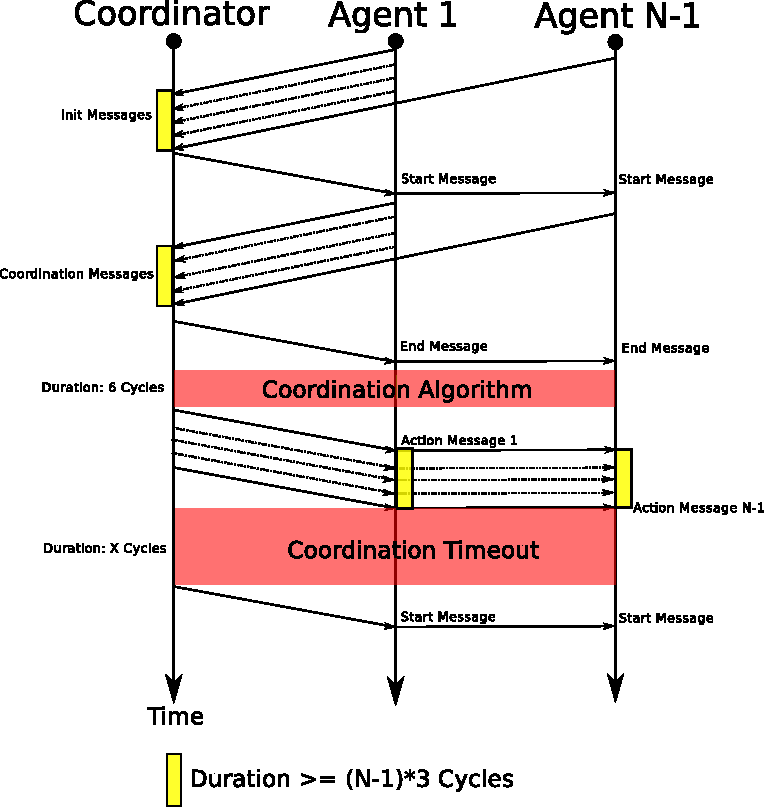
\includegraphics[width=0.8\textwidth]{Chapter4/figures/CoordComm.pdf}
  \caption{Communication Process in Coordination.} 
  \label{fig:coordinationprocess}
\end{figure}

Figure \ref{fig:coordinationprocess} shows the whole procedure of communication between the agents in order to coordinate their actions. First of all, agents have to initialize their presentation in the field with an ``init'' message. Goalkeeper saves these message in a temporal array and when he realizes that all players have been initialized themselves he sends them a ``start'' message. This message means that all players in the field are ready to start the coordination process. In this phase field players send their ``coordination'' messages to the goalkeeper. When goalkeeper gathers these messages from all field players, he sends them an ``end'' message to stop broadcasting. The next phase of the process is the execution of the coordination algorithm which lasts for six server cycles, approximately 120ms. After coordination phase calculated action must be sent to field players. We are using ``action'' messages to inform each player about the action he should do. After this phase, the same process is repeated after a timeout which can be defined by us.
%%%%%%%%%%%%%%%%%%%%%%%%%%%
\section{Coordination Beliefs}
In the above section we have presented about how field players exchange messages with the goalkeeper which is the coordination's administrator and the agent who executes the coordination's algorithm. In this section we are going to discuss about how the administrator could have the adequate knowledge of the world state receiving different observations from different agents. This is a field of major importance in such a multi agent system like simulation soccer. Having multiple observations of the same world could be a problem. Administrator has to combine all these observations without knowing which of them is faulty or correct in order to obtain a realistic representation of the world. Knowing ball's position and agents' positions will be more than enough to execute the algorithm without making guesses.

\subsection{Ball Position Weighted Samples}
Ball position is calculated only from agents' observation who are able to locate it in the field and have a good knowledge about their position as well. We can infer that these observations are obtained by agents who are sending ``type C'' coordination messages. Furthermore, if goalkeeper has also a ball observation he uses it too.
\begin{figure}[htb!]
\centering
  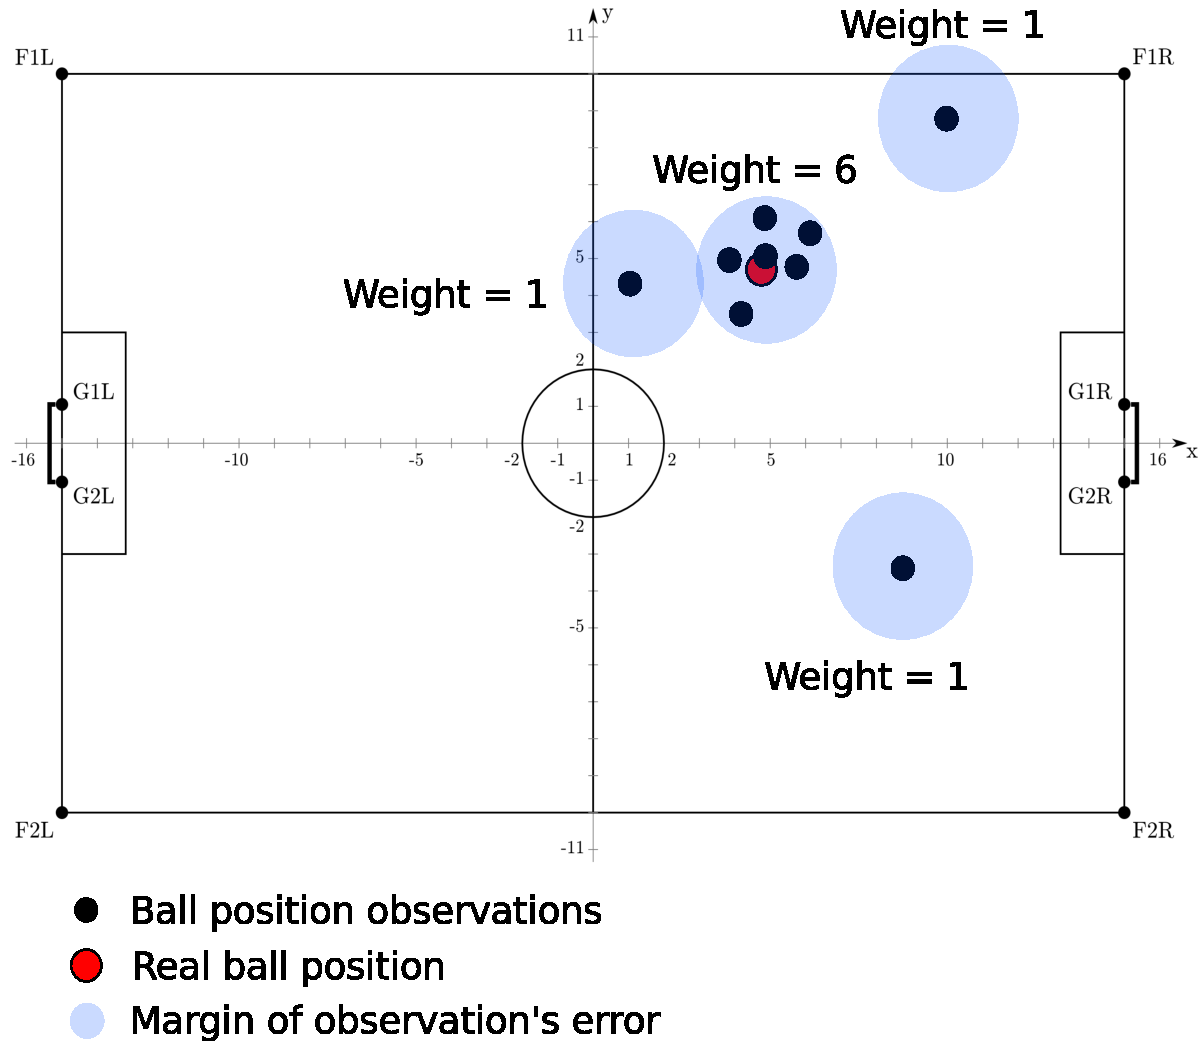
\includegraphics[scale=0.5]{Chapter4/figures/Ball.pdf}
  \caption{Ball's Position Observations.} 
  \label{fig:Ball}
\end{figure}
As we can see in Figure \ref{fig:Ball} ball observation can differ from each other. In our approach, we use a simple algorithm to approach ball's position with great accuracy. We use this algorithm to split these observations according to the others. A threshold is defined in order to form sets of observations. This threshold is called margin of observation error. Every observation set has a weight. In the beginning, for a given number of n observations we have n observation's sets each one of them has a default weight (1).\\
\\
${\bf Obsevation_{i} } = (x,y)$\\
${\bf Weight_{i}} = 1$\\
\\
Then, we try to correlate these sets, for every two sets which are been correlated it is formed a new set which contains observations from the two parent sets. The weight of the new set will be the sum of the parents' weight.\\
\\
${\bf Obsevation Set_{i} } = \lbrace (x_{1},y_{1}),...,(x_{k},y_{k}) \rbrace \vee k \in [1,n] , k\in \mathbb{Z}$\\
${\bf Weight_{i}} = k$\\
\\
Figure \ref{fig:Ball} shows the procedure. We can see four sets of observations which have been assigned a weight. The set with the most observations included is naturally assigned the biggest weight. Consequently, we have to calculate the final position of the ball.
Given N-observation's sets which each of them has K-observations, the final ball belief will be:\\
\\
${\bf Ball Belief} = \frac {1} {N} \displaystyle\sum\limits_{i=1}^N \frac {Weight_{i}} {N \ast K}  \displaystyle\sum\limits_{j=1}^K Obsevation Set_{i}[j]$
\subsection{Agent Distance from Ball}
The next step into beliefs section is to determine each agent's distance from the ball. This can be accomplished by two ways. First, for agents who send ``Type C'' and ``Type L'' coordination messages and they are able to know their exact position in the field, this distance is calculated by finding the distance between the ball and the agent. For players who are sending ``Type B'' coordination messages we just take the distance part of the message. Finally, for ``Type X'' messages we assume $\infty$ distance.

\section{Subsets in Coordination Process}
The existence of multiple operating agents makes coordination function is too complex or too expensive to solve by one single agent. In our case it would be the goalkeeper who is going to solve this huge problem for nine players or eleven which is the number of players in the next server's version. One possible solution to this problem is to split players into subsets which would be easier to coordinate their actions in real-time. In this approach, there are three subsets:
\begin{description}
\item[Active subset] Active subset consists of three agents. It is the most important set of agents in the coordination. Agents who constitute this subset have the responsibility of making worthy actions for their team. Moreover, having to calculate actions for three players is not complex for such an important group. 

\item[Support subset] Support subset consists of agents who are neither in the active subset nor the inactive one. Coordinate actions for these agents is the most time consuming and expensive part of the coordination algorithm.

\item[Inactive subset]Inactive subset consists of agents who are sending ``Type X'' messages. It is the less important set of agents in the coordination. Agents who constitute this subset assigned the same action, to find their position. Finding their positions will be resulted to be inserted either in the active or in the support subset in the next coordination cycle.
\end{description}

\section{Coordination Splitter}
In this section we are going to discuss how the above three groups are generated by coordination splitter. An array full of team's agents is sorted according to the distance each agent has from the ball. We assign to the active subset the agents in the three first positions of the sorted array.
Other agents with distance less than infinity join the support subset.
Remind that we assume $\infty$ distance from ball for the agents who have no idea for their position and have not the ball into the field of their view.
In Figure \ref{fig:Splitter} we can see an example of the coordination splitter. Assuming that all agents are complete awareness of their position, we could realize that the agents in the red distance's threshold will join the active subset. The other six players who have farther distance from ball will join the support subset.
\begin{figure}[htb!]
\centering
  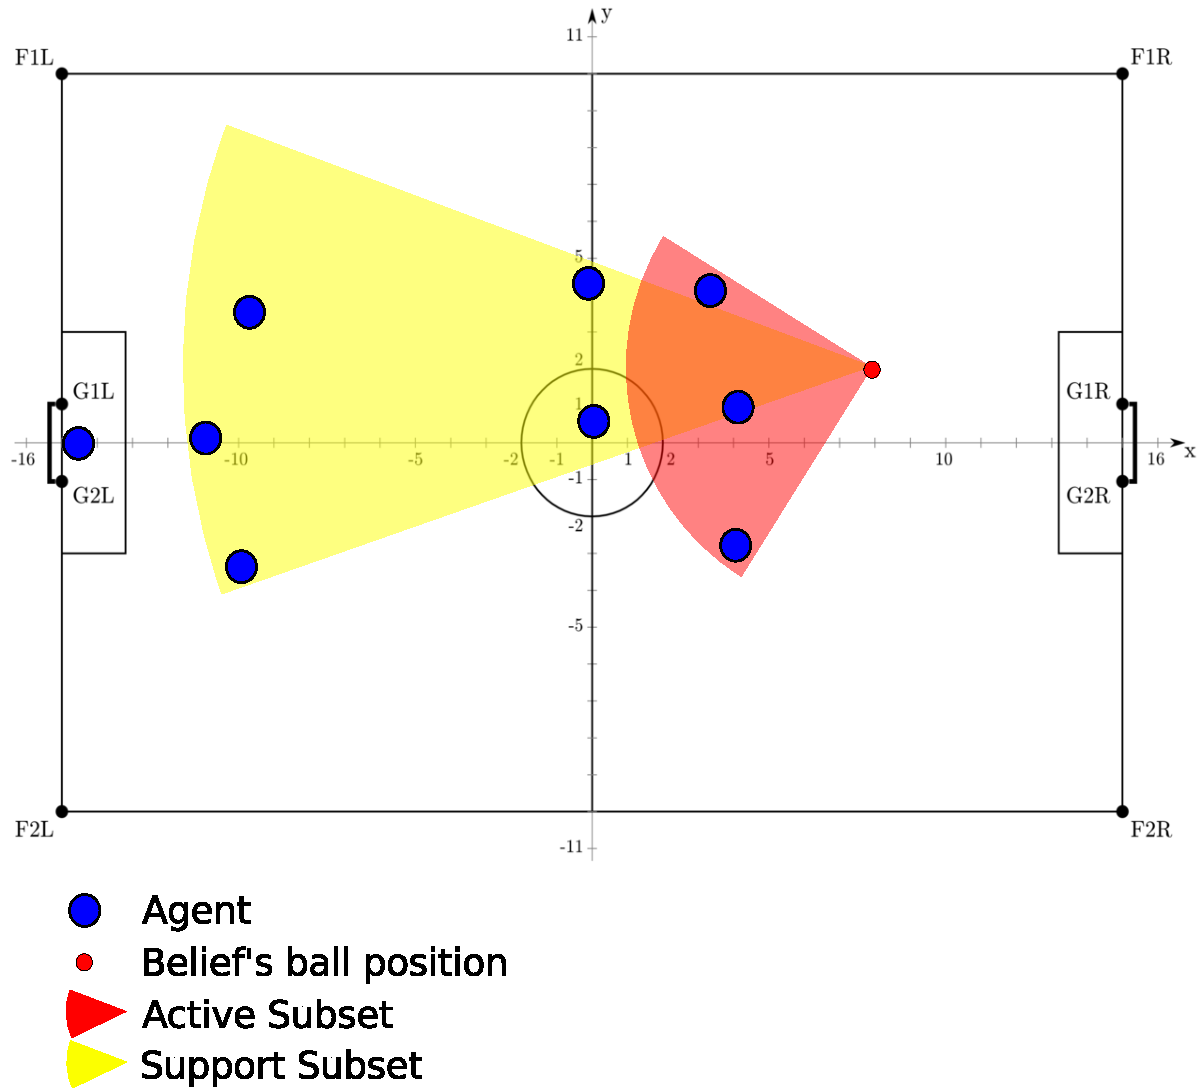
\includegraphics[width=\textwidth]{Chapter4/figures/Splitter.pdf}
  \caption{Coordination Splitter.} 
  \label{fig:Splitter}
\end{figure}

\section{Soccer Field Value}
\label{FieldValue}
In order to proceed with our discussion about coordination process, we have to demonstrate a simple but functional way to give a value in every spot of the soccer field. In Figure \ref{fig:SoccerValue} we see that each spot in the field takes a value from a function. The main idea is that as we ball is moving towards the opponent goal,  this value is becoming higher. In contrast as ball is moving towards our goal, this value is becoming lower.  
\begin{figure}[htb!]
\centering
  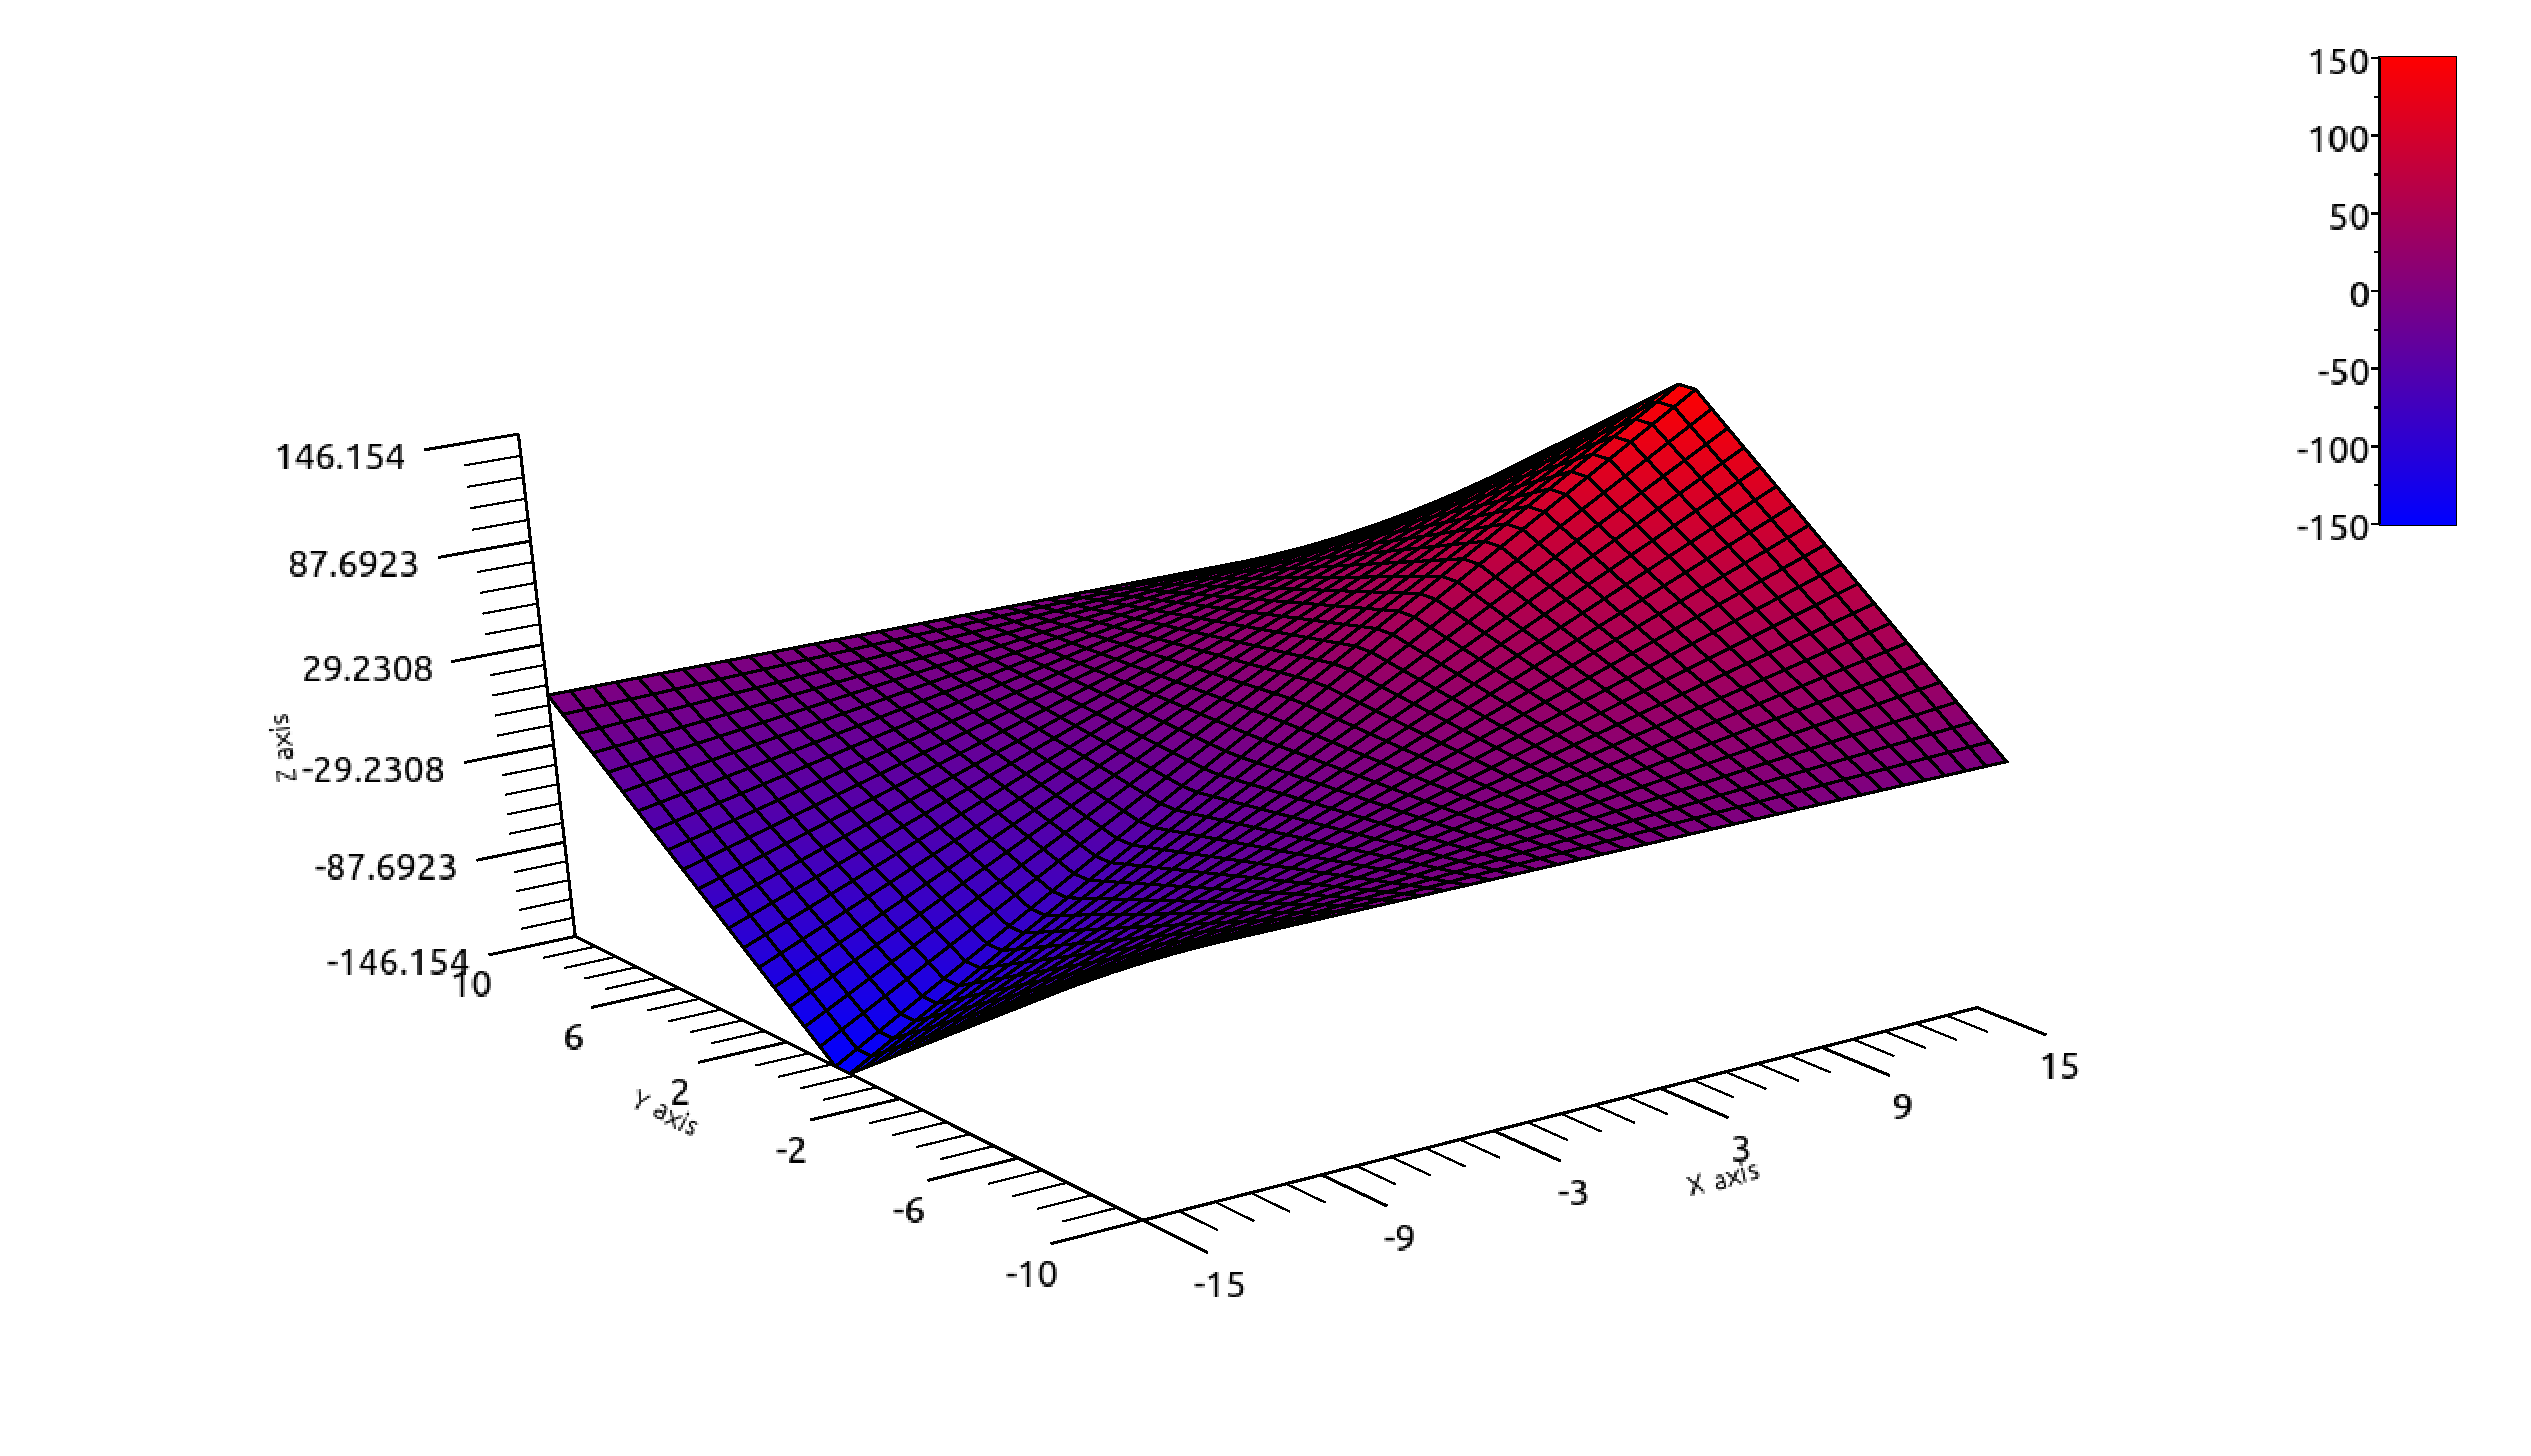
\includegraphics[width=\textwidth]{Chapter4/figures/Graph1.pdf}
  \caption{Soccer Field Value.} 
  \label{fig:SoccerValue}
\end{figure}

\section{Active-Positions Computation}
Until now, we have updated the coordination beliefs and we have split agents into subsets. in this phase of the coordination process, we have to find adequate and worthy positions for the active subset. We distinguish two cases, in the first case, ball is located in our field's half. In this case we have to find worthy positions which have a defensive approach. On the other hand, if ball is located in the other field's half we have to find positions which have an attacking approach. In both cases we create an array of equidistant coordinates which are located in a radius which is determined by the ball's location and they are not out of field's thresholds. Figure \ref{fig:ActivePositions2} shows how these positions are shown in the soccer field through roboviz monitor. 
\begin{figure}[htb!]
\centering
  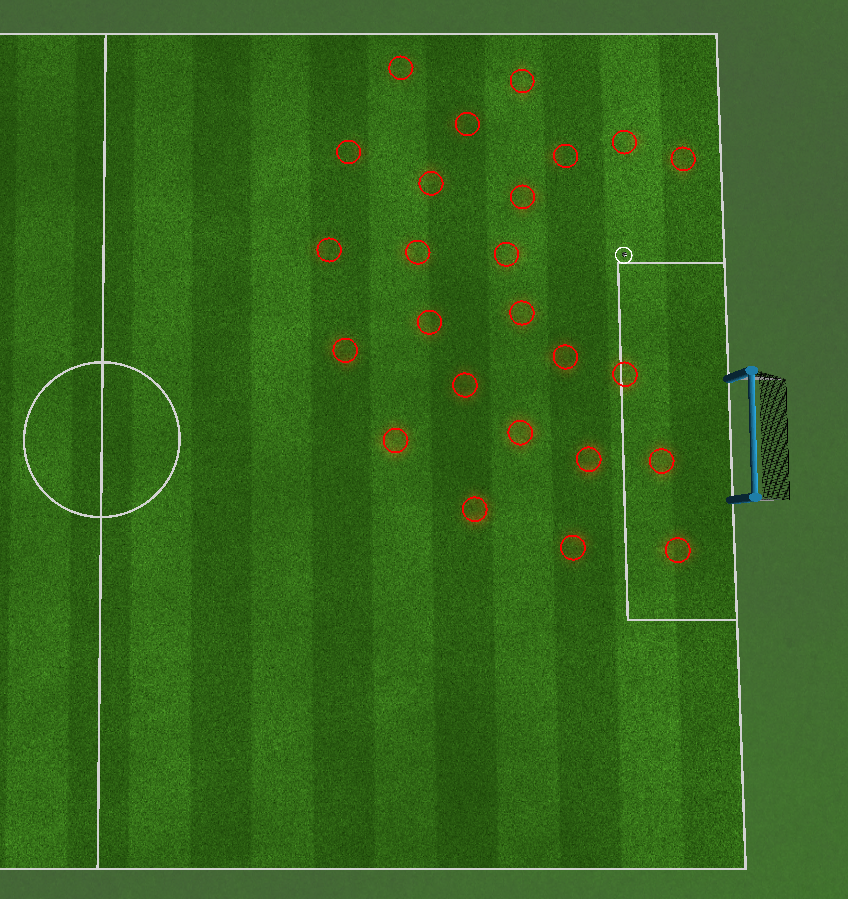
\includegraphics[width=7cm]{Chapter4/figures/ActivePositions2.png}
  \caption{Active positions before elimination.} 
  \label{fig:ActivePositions2}
\end{figure}

From these set of coordinates we choose the best according to their value. As we saw in the previous section each coordinate of the field has a unique value. Consequently, we will try to choose a number of coordinates which summarize in a max value in an attacking approach or in a min value in a defensive approach, careful not to overcome a max number of coordinates which is nine. This will help us to keep iterations below a threshold. Figure \ref{fig:ActivePositions3} shows how these positions are shown in the soccer field through roboviz monitor. 
\begin{figure}[htb!]
\centering
  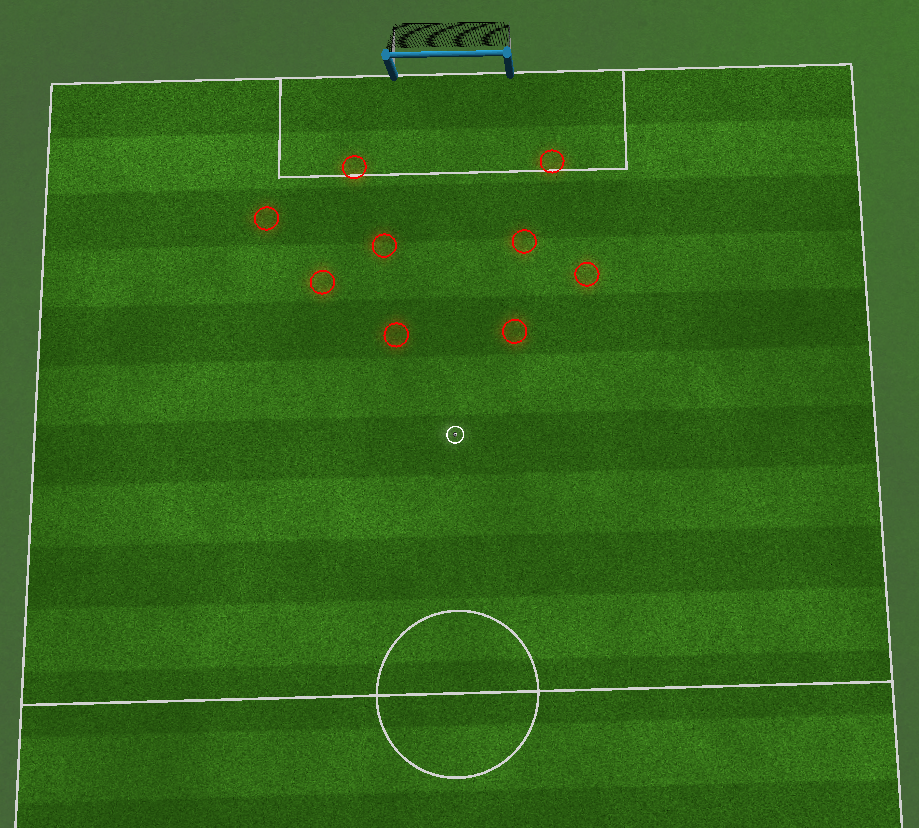
\includegraphics[width=7cm]{Chapter4/figures/Active3.png}
  \caption{Active positions after elimination.} 
  \label{fig:ActivePositions3}
\end{figure}


\section{Active-Subset Coordination}
Once we have find worthy positions for the active players it is time to find the player who is more adequate than others to become the on ball player. Moreover, we should assign each of the rest players into an active position. This is called mapping function and will have a significant role in the next coordination's phases. 
\subsection{Player on Ball}
An agent from the active subset has to be selected in order to be sent an action which is related to the ball. We have to find the agent who has minimum value according to two parameters:
\begin{enumerate}
\item \textbf{Distance from ball} $d_{i}$, ball's distance from each agent in the subset. 
\item \textbf{Angle towards goal} $\vartheta_{i}$, this angle is the sum of two angles, the first is the angle between agent's body and the ball. The other angle is the angle between ball and the opponent's goal.
\end{enumerate}
Given an active subset:\\
${\bf ActiveSubset} = \lbrace Agent_{1},Agent_{2},Agent_{3} \rbrace $\\
${\bf Value_{i}} = d_{i} + a \ast \vartheta_{i}, a\in\mathbb{R}$\\
${\bf OnBallPlayer} = \arg\min_{i}(Value_{i}) $\\
\\Additionally, we give to the agent who had been assigned an action towards the ball in the previous coordination cycle a small
advantage over the others to be again the on ball player. We do this due to the fact that there will be continuously changes in the on ball player in cases in which two agents have approximately same distances and angles from the ball.
\subsection{Active-Subset Best Mapping}
Next in the active coordination phase we should assign positions for the other two players who have been included to the active subset. Algorithm \ref{ActiveMapping} shows how we can find the optimized mapping. In a greedy approach, we calculate the cost of every possible mapping. In addition, in every mapping we take into account the following mapping $(OnBallPlayer \rightarrow Ball)$ which will be helpful in order to find possible collisions between on ball and the active players. Given a set of nine positions the active coordination algorithm will be:
\begin{algorithm}[htb!]
\caption{Active-Subset Best Mapping}
\label{ActiveMapping}
\begin{algorithmic}[1]
\STATE {\bf Inputs: }$ActivePlayers = ActiveSubset - Agent_{OnBall} $
\STATE $Activepositions = \lbrace P_{1},P_{2},...,P_{N} \rbrace $
\STATE {\bf Outputs: }$OptimActiveRoleMap$
\STATE $OptimActiveRoleMap = \varnothing $
\STATE $S = {{N}\choose{2}}$
\FOR{{\bf each} s in S}
\STATE $ActiveRoleMap = RoleMap[s] \cup (OnBallPlayer \rightarrow Ball)$
\STATE $OptimActiveRoleMap = mincost(ActiveRoleMap,OptimActiveRoleMap)$
\ENDFOR
\end{algorithmic}
\end{algorithm}
We can realize that even we are using a brute force method the number of possible mapping remains able to be computed in real-time. Assuming maximum number of active positions in our case nine, the possible mappings are: ${{9}\choose{2}} = 72$ mappings.

\section{Team Formation}
The formation itself is not a main contribution of this thesis but serves to set up the role assignment function and the coordination of the support subset. In general, team's formation is determined by the ball's position in the field. The formation is broken up into three groups including all players of the team except from goalkeeper.This section presents the team's formation used in our approach for both 0.6.5 and 0.6.6 rcssserver3d versions.
\subsection{9-Players Server Version (0.6.5)}
Attacking group which consists of three positions:
\begin{description}
\item[FC] \textit{Forward center}
\item[FL] \textit{Forward left}
\item[FR] \textit{Forward right}
\end{description}
Defensive group which consists of three positions:
\begin{description}
\item[DC] \textit{Defender center}
\item[DR] \textit{Defender right }
\item[DL] \textit{Defender left}
\end{description}
Finally, midfield group which consists of two positions:
\begin{description}
\item[ML] \textit{Midfielder left}
\item[MR] \textit{Midfielder right}
\end{description}
As an example, Figure \ref{fig:Formation9_0} shows how the different role positions of the formation are depicted in the soccer pitch. In general attackers are responsible to be assigned positions near to ball when ball is on opponents' half of the field. Then, the forward center  is given a position close to the ball and the other two forwards are given positions on either side of the ball in an angle and a distance offset which are determined and dynamically changed according to the ball's exact coordinate. If ball is located in our half, then forwards are given positions which are in the middle of the field. On the other hand, defenders are mainly positioned to guard our goal. To determine their position on the field a straight line is calculated between of the team's own goal and the ball. Central defender is given a position placed on this line and his distance from our goal is proportional to the ball's position. The other two defenders' positions are located on either side of the defender center. Midfielders' positions is determined by the ball's position as well. For an attacking phase, in which ball is located to the opponents' half of the pitch, midfielders are given position near to the forwards in order to support our attack. In the opposite situation they are given position in front of our defense line to help defenders. Finally, goalkeeper positions himself independently to always be in the best position to stop a shot towards our goal. In some cases, when ball is located near to the field's edges formation positions are adjusted not to be out of them.
\begin{figure}[htb!]
\centering
  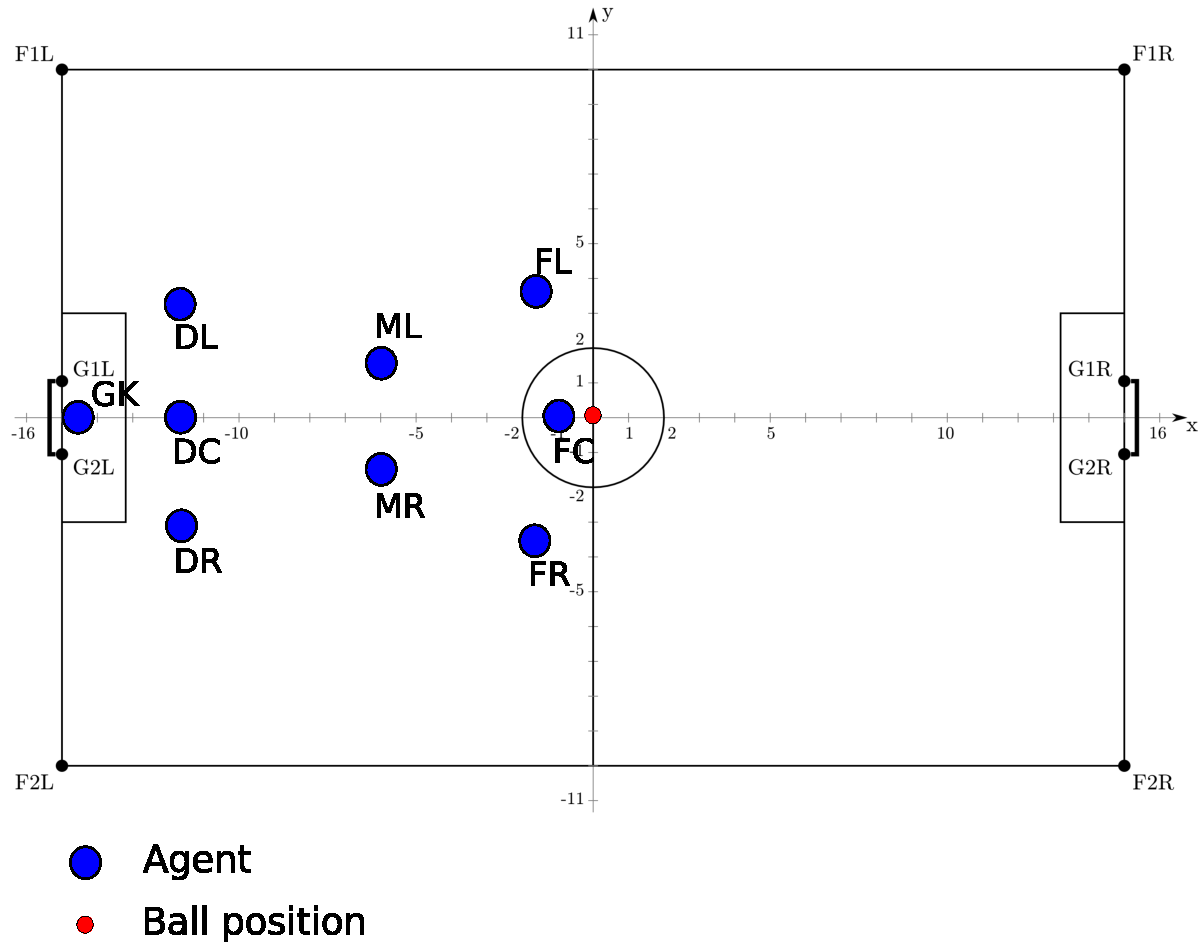
\includegraphics[width=\textwidth]{Chapter4/figures/Formation9_0.pdf}
  \caption{Formation Role Positions for 9 vs 9.} 
  \label{fig:Formation9_0}
\end{figure}

\subsection{11-Players Server Version (0.6.6)}
Attacking group which consists of four positions:
\begin{description}
\item[FC] \textit{Forward center}
\item[FL] \textit{Forward left}
\item[FR] \textit{Forward right}
\item[SF] \textit{Support Forward}
\end{description}
Defensive group which consists of three positions:
\begin{description}
\item[DC] \textit{Defender center}
\item[DR] \textit{Defender right }
\item[DL] \textit{Defender left}
\end{description}
Finally, midfield group which consists of two positions:
\begin{description}
\item[MC] \textit{Midfielder center}
\item[ML] \textit{Midfielder left}
\item[MR] \textit{Midfielder right}
\end{description}
\begin{figure}[htb!]
\centering
  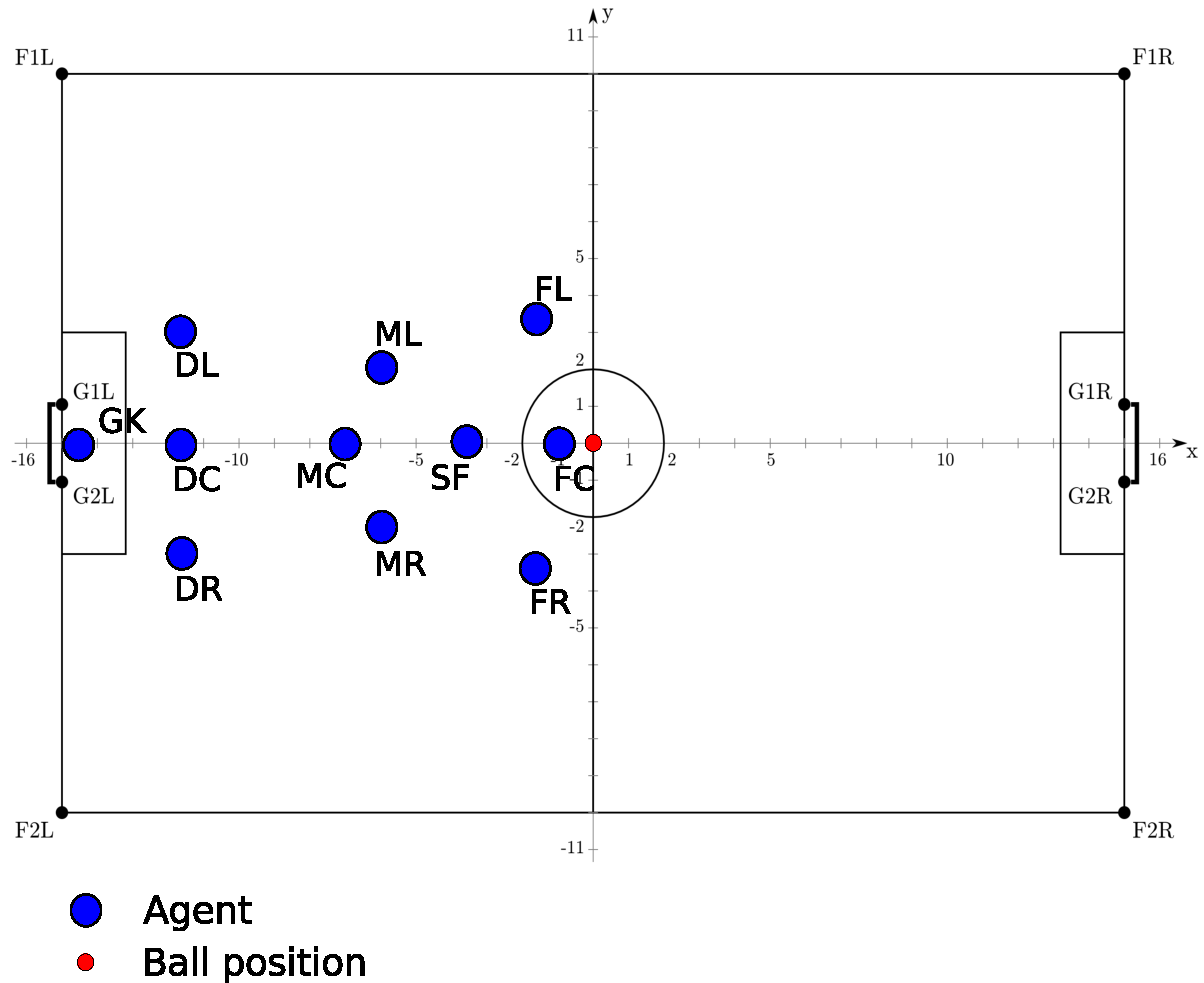
\includegraphics[width=\textwidth]{Chapter4/figures/Formation11_0.pdf}
  \caption{Formation Role Positions for 11 vs 11.} 
  \label{fig:Formation11_0}
\end{figure}
Figure \ref{fig:Formation11_0} depicts how the different role positions of the formation shown in the soccer pitch for the newer server version in which team consists of eleven players. Forward group is based on the same principle as the previous version's approach. In addition, a player is added beyond the forward center's position. In the midfield region there are now three players. Midfield center's position is behind with an offset distance from the forward center's position. Moreover, the other two midfielder positions are on either side of the midfield center position in an angle and distance. Defense line is exactly the same as it was in the previous version.

\section{Role Assignment Function}
In this section we present the role assignment function. This function after the evaluation of the current game state's beliefs and the optimized active positions, tries to assign roles for the all agents. This will prove to be very helpful on the next coordination steps when we will have to find positions for the support subset's agents. Given a calculated team formation we have to assign roles to the active subset's players. As we know, positions for active agents are strictly connected and near to the ball's position on the field. So, for N active players we choose N team's formation positions which minimize the distance from the ball. These team's formation roles will be assigned to the active players. The other team roles will be available to the support subset during support coordination process. As an example, figure \ref{fig:RoleAss} shows how the this role assignment works. Active players will be assigned the red team roles due to the fact that they are located near to the ball's position. Once these positions will be bound by the active players, the only roles that support players can compete about will be the grey colored positions. A naive role mapping would have assign roles permanently to specific players. This will be performed poorly in such a dynamic environment. It would be also weak in situations where an agent assigned to a defensive role may end up out of position without being able to change roles with another player who may be in a better position to defend our goal. In our approach, every role mapping is calculated with a full sense of the world's state, resulting to a dynamic and unpredictable way of assigning roles to the agents. During testing, there were several cases in which a forward player ended up to have a defense role at the end of the game or the opposite.
\begin{figure}[htb!]
\centering
  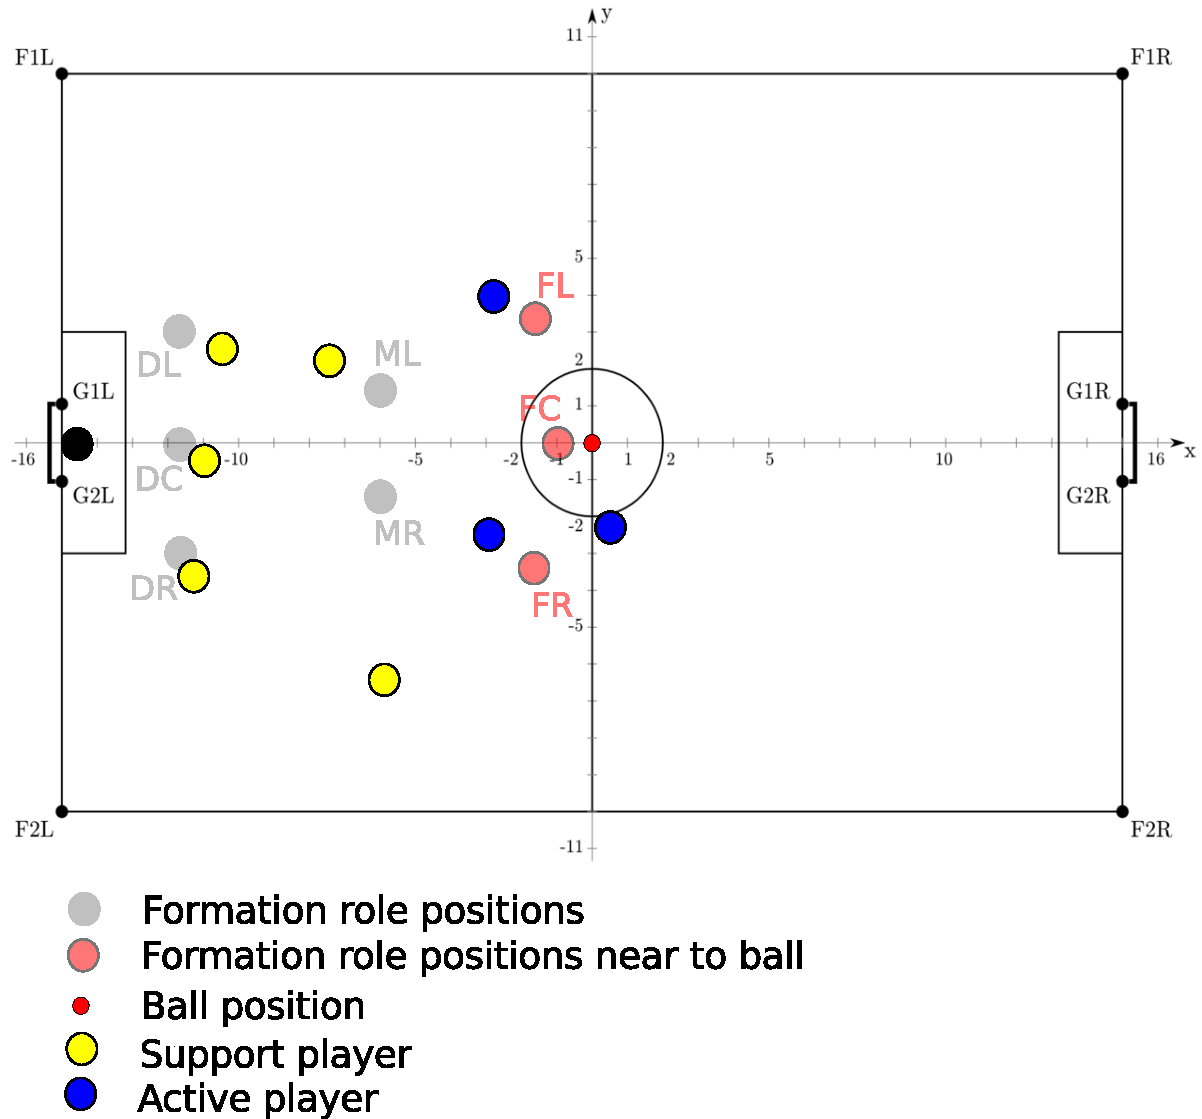
\includegraphics[width=0.8\textwidth]{Chapter4/figures/RoleAss.pdf}
  \caption{Role Assignment Function.} 
  \label{fig:RoleAss}
\end{figure}


\section{Positions for Support-Subset}
In this section, we are going to discuss about which position will assigned to the support subset. In an ideal case, we would have same number of support agents and same number of positions, this is going to happen when inactive subset is completely empty. In this case this section has not any meaning. In other cases, when there are agents who are not able to know their positions or seeing ball, we have to decide about which position of the team's formation will be eliminated from the support coordination. Considering the ball's position, we have to make sure that there will be positions for support players near to the ball. So, given N players in the support subset we simply compare these team's formation position to find the N closest to the ball's positions. Coordination's final step will find an optimized way to map support agents to these positions.
\begin{figure}[htb!]
\centering
  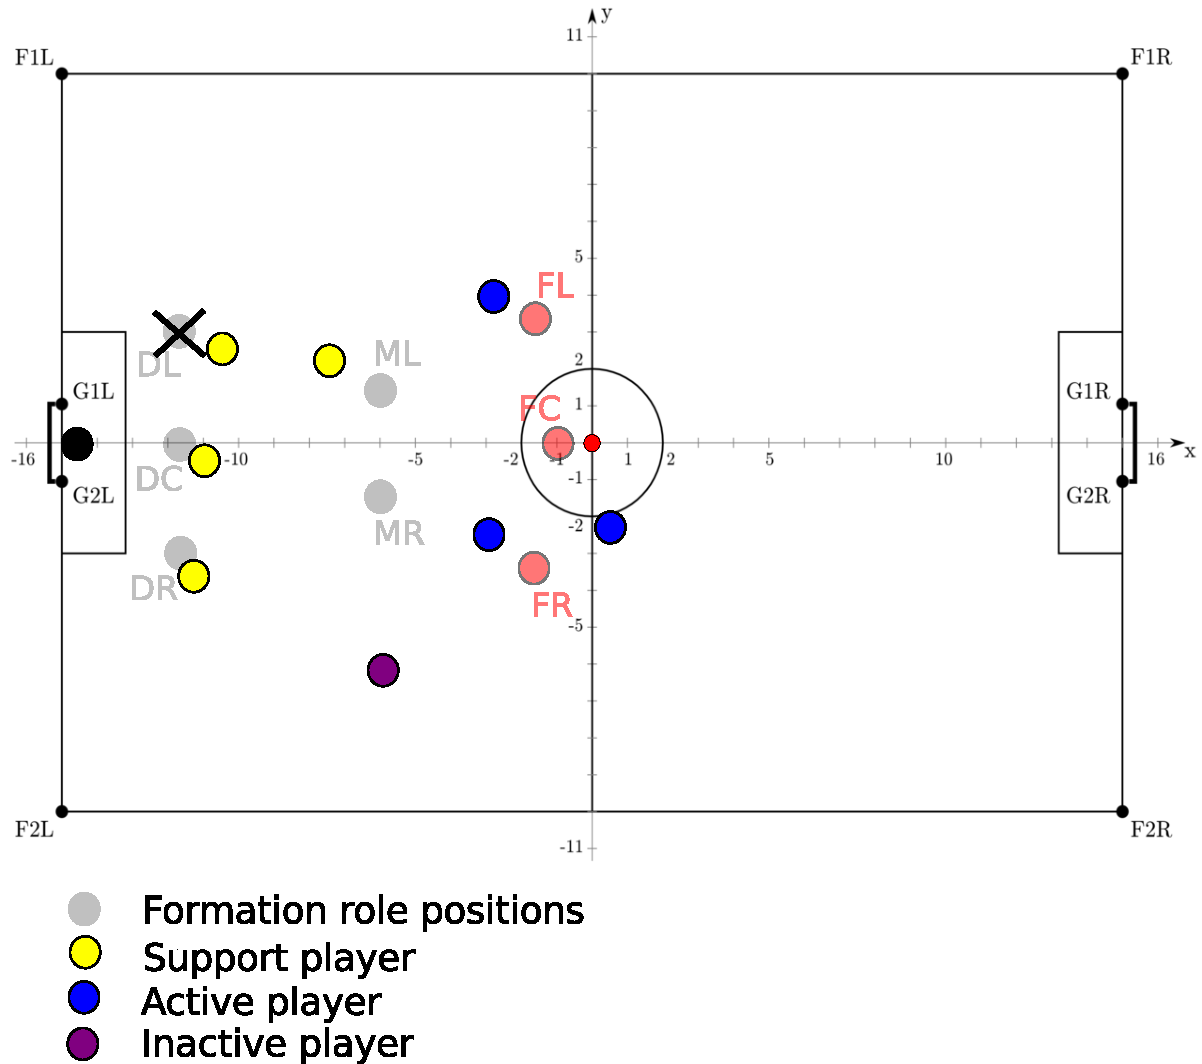
\includegraphics[width=0.8\textwidth]{Chapter4/figures/SupportPos.pdf}
  \caption{Support Positions.} 
  \label{fig:SupportPos}
\end{figure}

\section{Support-Subset Coordination}
This is the final phase of the coordination process. Until, now we have calculated the optimal mapping of the active agents' subset. So it's time to find a mapping which will give as an optimal solution for the support agents as well. Given a support position set which has been discussed in the previous two sections we have to assign a position of this set to each and every agent of the support subset. Using a greedy algorithm which would calculate all possible mapping to find the optimal solution was the first solution to this problem. However, a brute force approach would only be applicable for the previous server's version in which each team consists of nine players, in which we would have to calculate all mappings only for the support subset which consists of five players at maximum. This means a factorial complexity about: $\leqslant 5! \Leftrightarrow  {{5}\choose{5}} = 120$ mappings. Unfortunately, moving from nine to eleven eleven players this would be a problem as having to calculate at worst case $ 7! \Leftrightarrow  {{7}\choose{7}} = 5040$ mappings it would be difficult for an agent to calculate all these mappings in real-time without any delay in sending effector messages to the server. We find the solution in a UT Austin Villa's paper \cite{UtAustinVillaPaper} which was appeared in the RoboCup international Symposium. A dynamic programming implementation which is able to compute an optimal solution within the time constraints imposed by the decision cycle's length ($\approx$ 20ms ).
\begin{algorithm}[htb!]
\caption{Dynamic programming implementation \cite{UtAustinVillaPaper}}
\label{alg3}
\begin{algorithmic}[1]
\STATE {\bf Inputs: }$SupportPlayers = \lbrace A_{1},A_{2},...,A_{n} $
\STATE $SupportPositions = \lbrace P_{1},P_{2},...,P_{n} \rbrace $
\STATE {\bf Outputs: }$OptSupportMap$
\STATE $OptSupportMap = \varnothing $
\FOR{$k = 1 \to n$} 
\FOR{{\bf each} $\alpha$ in SupportPlayers}
\STATE $ S = {{n-1}\choose{k-1}} $, sets of k-1 agents for supportPlayers - $\lbrace \alpha \rbrace$
\FOR{{\bf each} s in S}
\STATE $SupportRoleMap$ $m_{0}$ = $RoleMap[s]$
\STATE $SupportRoleMap$ $m$ = $m_{0}$ $ \cup (\alpha \rightarrow P_{k})$
\STATE $OptSupportMap[\lbrace \alpha \rbrace \cup s] = mincost(m,OptSupportMap[\lbrace \alpha \rbrace \cup s])$
\ENDFOR
\ENDFOR
\ENDFOR
\end{algorithmic}
\end{algorithm}

This dynamic Algorithm \ref{alg3} is based on a key recursive property, theorem \ref{Theorem 1}.  This property stems from the fact that for every mapping there is a subset of a lower cost with which we can reduce the cost of the complete mapping by augmenting  it with that of the subset's lower cost mapping. An example of this procedure is shown in Table \ref{tab:DynamicTable}. As we see in this table, an optimal mapping is built iteratively for position sets from $\lbrace P_{1} \rbrace$ to $\lbrace P_{1},P_{2},...,P_{n} \rbrace$. In every step of this algorithm we use the lower cost's mapping for a subset of agents and positions which are compatible with our current mapping.



\begin{table}[htb!]
\label{tab:DynamicTable}
\centering
    \begin{tabular}{ | l | l | l | p{5cm} |}
    \hline
    $\lbrace P_{1} \rbrace$   & $\lbrace P_{1},P_{2} \rbrace$ 	& $\lbrace P_{1},P_{2},P_{3} \rbrace$\\ \hline
    $A_{1} \rightarrow P_{1}$ & $A_{1} \rightarrow P_{2},min(A_{2} \rightarrow P_{1})$	 	& $A_{1} \rightarrow P_{3},min(\lbrace A_{2},A_{3} \rbrace \rightarrow \lbrace P_{1},P_{2} \rbrace)$  \\ \hline
    $A_{2} \rightarrow P_{1}$ & $A_{1} \rightarrow P_{1},min(A_{3} \rightarrow P_{1})$	 	& $A_{2} \rightarrow P_{3},min(\lbrace A_{1},A_{3} \rbrace \rightarrow \lbrace P_{1},P_{2} \rbrace)$  \\ \hline
     						  & $A_{2} \rightarrow P_{2},min(A_{1} \rightarrow P_{1})$ 		& $A_{3} \rightarrow P_{3},min(\lbrace A_{1},A_{2} \rbrace \rightarrow \lbrace P_{1},P_{2} \rbrace)$  \\ \hline
       						  & $A_{2} \rightarrow P_{2},min(A_{3} \rightarrow P_{1})$ 		&   \\ \hline
       						  & $A_{3} \rightarrow P_{2},min(A_{1} \rightarrow P_{1})$ 		&   \\ \hline
    						  & $A_{3} \rightarrow P_{2},min(A_{2} \rightarrow P_{1})$		&   \\
    \hline

    \end{tabular}
    
    \caption{Mappings Evaluated During Dynamic Algorithm \cite{UtAustinVillaPaper}.}    
\end{table}

Remind that in the \textit{Kth} iteration of the algorithm, each agent will be assigned to the $P_{K}$ position. Then the possible positions K-1 will be assigned to the other n-1 agents. These assignments result in a total of $ {{n-1}\choose{k-1}} $ mappings to be evaluated each in each iteration. Summing to $\sum\limits_{i=1}^N{{n-1}\choose{k-1}}$ possible mappings.\\
\begin{center}
$\sum\limits_{i=1}^N{{n}\choose{k-1}}$ = $\sum\limits_{i=0}^{n-1}{{n-1}\choose{k}}$ = $2^{n-1}$
\end{center}
Therefore, the total number of mappings that we have to calculate their costs using this approach are $n2^{n-1}$. For nine players in each team this algorithm would not have any impact in making coordination faster as the previous brute force algorithm will have 5! (120 mappings) not much bigger complexity than this approach $5 \ast 2^{4}$ (80 mappings). However, in the new version of soccer simulator in which we can have even seven players in our support subset this approach gives us great improvement in our coordination time, $7 \ast 2^{6}$ (448 mappings) $\ll$ 7! (5040 mappings).

\section{Mapping Cost Computation}
In this section we are going to present how each mapping's cost is calculated. This function serves our approach in two cases. First, in active coordination in which active players wants to find an optimized mapping between them and the possible active position. Second, in support coordination in which support players wants to find an optimized mapping between them and the team's formation position which have assigned to them.

\subsection{Properties for Support-Subset Mapping Cost}
For support players things were easy. In support coordination we have same number of agents and positions. So these properties are:  
\begin{enumerate}
\item \textbf{Total distance }$C_{d}$ - Total distance agents have to travel in order to reach in their optimized mapping positions. It is a positive cost, so agents will try to minimize this cost.
\item \textbf{Possible Collisions }$C_{c}$ - In each mapping we check every combination of two agents and their assigned position if are to collide. If the lines between agents and their target positions are intersecting in a point which has almost the same distance from the agents then we add a big cost in this mapping. It is a positive cost and agents will try to minimize it. Figure \ref{fig:AvoidCollision} shows the idea behind the detection of a possible collision between two agents. In order to detect a possible collision these two distances $d_{1}$,$d_{2}$ have to have a small difference between them.
\begin{figure}[htb!]
\centering
  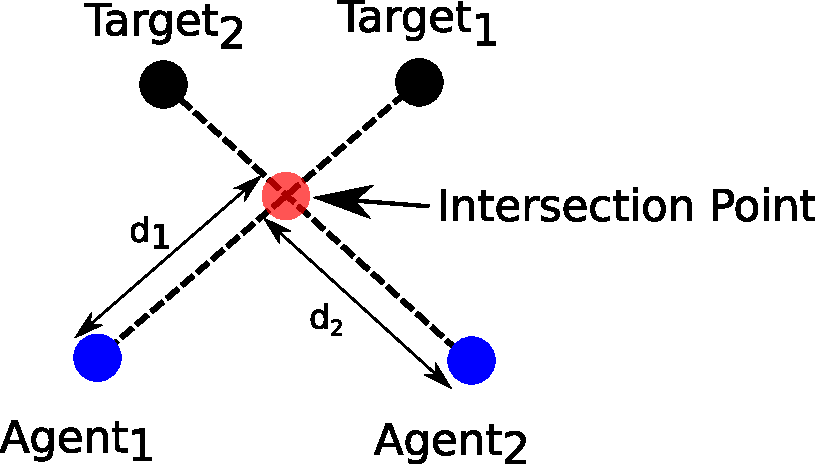
\includegraphics[width=0.5\textwidth]{Chapter4/figures/AvoidCollision.pdf}
  \caption{Collision Detection Approach.} 
  \label{fig:AvoidCollision}
\end{figure}
\end{enumerate}
\begin{center}
$Total cost = C_{d}+C_{c}$
\end{center}
As you can realize, the mapping with the smallest cost will be chosen by coordination's executor.

\subsection{Properties for Active-Subset Mapping Cost}
In active coordination we have two agents and a maximum of nine positions. It is obvious that we have to take into consideration more properties. Using the same support's properties will force our players to go always to the nearest positions. So, we had to think about other properties in order to assign target positions for our players which will be valuable for the team's defensive and offensive movement without the ball. These properties are shown below:
\begin{enumerate}
\item \textbf{Total distance }$C_{d}$
\item \textbf{Field's value }$C_{v}$ - Agents will try to maximize this cost according to the game state and the value which has every position in the field, see Section \ref{FieldValue}. For example, in an attacking phase agents will try to select positions which maximize this value. It is a negative cost.
\item \textbf{Possible Collisions }$C_{c}$
\item \textbf{Close routes }$C_{r}$ - Agents routes should be safe, so we calculate the difference between start positions' distance and target positions distance. This cost is a negative cost and agents will try to maximize this.
\item \textbf{Neighboring positions }$C_{p}$ - In general agents will try to avoid be assigned in neighboring positions. So if their target positions are near to each other this is going to add more cost. It is a negative cost and agents will try to maximize this.
\item \textbf{Positions aligned to X-axis }$C_{a}$ - we want team stretching into the field in order to have players in all regions of the soccer pitch. Agents will try to maximize their Y-axis difference and this cost is negative too. 
\end{enumerate}
\begin{center}
$Total cost = C_{d}-C_{v}+C_{c}-C_{r}-C_{p}-C_{a}$
\end{center}
The same principle applies here too, the mapping with the smallest cost will be chosen by coordination's executor.